\newpage
\section{Wyniki}

Parametry modelu:
\begin{itemize}
	  \item liczba neuronów warstw ukrytych - $100$
	  \item liczba warstw - $2$
	  \item liczba głowic - $100$
	  \item rozmiar batcha - $40$
	  \item czas uczenia - $40h$
	  \item Liczba epok - $6$
	  \item współczynnik uczenia - $0.004$
	  \item liczba kroków czasowych - $50$
	  \item skuteczność - $5\%$
	\end{itemize}
	
Nie udało nam się otrzymać wyników zbliżonych do tych osiągniętych podczas konkursu PAN. Sprawdziła się
część elementów z analizy ryzyka, które przewidywaliśmy.

\subsection{Problemy}
\subsubsection{Małe doświadczenie w dziedzinie konstruowania sieci neuronowych}
Było to dla nas pierwsze doświadczenie z sieciami neuronowymi, dlatego znaczną ilość czasu poświęciliśmy na 
zrozumienie tego zagadnienia. Aby zrozumieć samą ideę zaczęliśmy od prostych modeli sieci typu feed forward,
następnie przeszliśmy do sieci rekurencyjnych. W całym procesie nauki musieliśmy zrozumieć,
wszystkie zagadnienia z nimi związane, jak etropia krzyżowa, softmax, propagacja w przód, propagacja wsteczna, 
minimalizacja gradientu itp.
 
\subsubsection{Długi czas uczenia}
Jedna epoka trwała od kilku do kilkunastu godzin w zależności od ilości danych, co znacząco spowalniało 
prace nad usprawnieniem modelu. 
 
\subsubsection{Znajomość biblioteki}
Zdobytą wiedzę i pomysł należało przełożyć na kod w Pythonie przy wykorzystaniu biblioteki Pytorch. 
Problem, który rozwiązywaliśmy był w jakimś stopniu niestandardowy, dlatego należało modyfikować 
gotowe narzędzia i odpowiednio komponować z nich kod, często popełniane przy tym błędy prowadziły 
do bardzo stopniowych zmian w kodzie, które oddzielone były długim czasem uczenia na sprawdzenie poprawek.

\subsubsection{Przeuczenie}
Ze względu na specyfikę problemu, którego cechą są bardzo krótkie teksty wejściowe bardzo poważnym 
problemem jest przeuczenie sieci, która
bardzo szybko uczy się tekstów treningowych na pamięć. 

\subsubsection{Różnice w długości tekstów}
Teksty są bardzo krótkie, dodatkowo różnią się długością. Teksty mają od 1500 do 2600 znaków. 1100 znaków 
różnicy w tym przypadku to aż $43\%$ różnicy w długości. Teoretycznie głowica powinna uczyć się przewidywać znaki dla 
swojego autora i na tekstach treningowych robić to najlepiej w porównaniu do pozostałych głowic dla tekstu 
jej autora ze zbioru testowego. Problemem jest jednak sytuacja wyżej opisana. Kiedy znaków jest tak mało 
możliwa jest sytuacja w której głowica, której teksty są tymi najdłuższymi lepiej uczy się modelu języka od
pozostałych głowic więc skuteczniej przewiduje kolejne znaki dla wszystkich nieznanych teksów.

Popularne modele, które potrafią przewidywać kolejne słowa bądź litery szkolone są przykładowo na danych w postaci licznych 
artykułów z \texttt{Wikipedii}, gdzie liczba danych do wyczuenia jest znacznie większa.

\subsubsection{Błędy implementacyjne}
Błędy w implementacji sieci, które prowadziły do skrajnie złych wyników i znacznie opóźniały tempo pracy.
\begin{figure}[H]
	\centering
	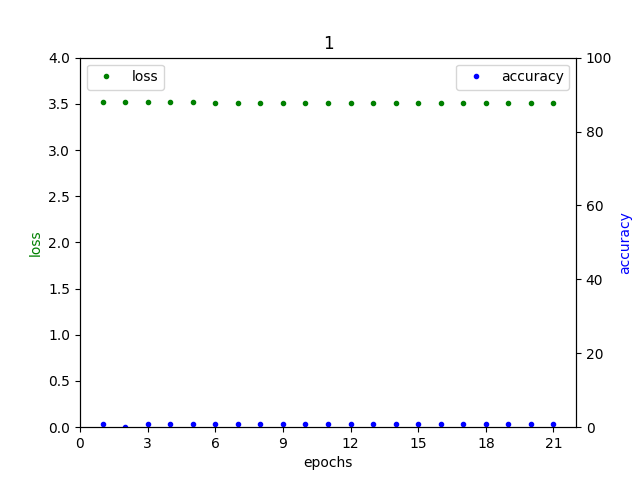
\includegraphics[height=7cm]{./images/result1.png}
	\caption{przykładowe dane z uczenia sieci błędnie zaimplementowanej}
	\label{fig:test5}
	\end{figure}

\subsection{Wyniki eksperymentów i debugowanie sieci}
Niestety nie udało nam się otrzymać pozytywnych wyników. Został popełniony błąd w implementacji sieci,
którego nie udało nam się wykryć i rozwiązać. Efektem tego było to, że sieć się nie uczyła, a potem kiedy zaczęła się 
uczyć nadal miała bardzo niską skuteczność na danych testowych. Głównym problemem był tu czas ewaluacji. 
Debugowanie prowadziliśmy etapami, sprawdzając kolejne elementy sieci. Wyróżniliśmy następujące:

\subsubsection{Sprawdzenie modułu preprocesingu}
	Jest to najbardziej obszerny moduł. Podejrzewaliśmy, że problem może wynikać ze złego kodowania znaków,
	na przykład wszystkie znaki są zakodowane identycznie i stąd sieć się nie uczy. W tym celu odkodowywaliśmy
	zakodowane teksty i wyświetlaliśmy je na ekran. Jak się okazało teksty były zakodowane poprawnie, włączając w
	to redukcję alfabetu. Przykład:
	
	Oryginalny tekst:
	\begin{bash}
 Sir, you are sad! The silent eloquence
 Of yonder tear that trembles on your eyelash
 Proclaims a sorrow far more deep than common;
 Confide in me--fear not--I am a mother!
	\end{bash}
	
	Tekst po odkodowaniu: 
	\begin{bash}
sir, you are sad! the silent eloquence
of yonder tear that trembles on your eyelash
proclaims a sorrow far more deep than common;
confide in me--fear not--i am a mother!
	\end{bash}
	Widać zmapowane duże znaki na małe. Jest to zachowanie oczekiwane.
	
\subsubsection{Sprawdzenie modułu batchowania}
	  Jest to bardzo obszerny moduł, który czyta dane z tensorów zapisanych na dysku
	  i na ich podstawie generuje kolejne batche, podając kolejnych autorów w możliwie losowej kolejności, tak by sieć
	  nie uczyła się artefaktów. Generuje przy tym oczekiwane wyjście, które następnie jest wykorzystywane do 
	  liczenia kosztu. Ilość błędów do popełnienia przy tego typu module była bardzo duża i nie wykluczalaliśmy
	  żadnego scenariusza. Upewniliśmy się, że:
	\begin{itemize} 
	  \item {autorzy są podawani w losowej kolejności - poprzez sprawdzenie metody losującej numery autorów,
	  a takze poprzez wypisywanie na ekran autorów w kolejnych batchach}
	  \item {moduł ``przechodzi'' po tekstach poprawnie - to znaczy, czy kolejne sekwencje podawane do sieci to 
	  kolejne litery danego autora - w tym celu odkodowywaliśmy z batcha wektory one hot przy pomocy 
	  specjalnie przygotowanego skryptu. Odkodowywaliśmy także oczekiwanie wyjście. Żeby wykluczyć ewentualne błędy
	  teksty były odkodowywane wykorzystując alfabet poprzez który były kodowane.
	  Przykład dla jednego autora:
\begin{bash}
AUTHOR 0) SEQUENCE: |my, my, i was forget|     TARGET: |t|
AUTHOR 0) SEQUENCE: |y, my, i was forgett|     TARGET: |i|
AUTHOR 0) SEQUENCE: |, my, i was forgetti|     TARGET: |n|
AUTHOR 0) SEQUENCE: | my, i was forgettin|     TARGET: |g|
AUTHOR 0) SEQUENCE: |my, i was forgetting|     TARGET: | |
AUTHOR 0) SEQUENCE: |y, i was forgetting |     TARGET: |a|
AUTHOR 0) SEQUENCE: |, i was forgetting a|     TARGET: |l|
AUTHOR 0) SEQUENCE: | i was forgetting al|     TARGET: |l|
AUTHOR 0) SEQUENCE: |i was forgetting all|     TARGET: | |
AUTHOR 0) SEQUENCE: | was forgetting all |     TARGET: |a|
AUTHOR 0) SEQUENCE: |was forgetting all a|     TARGET: |b|
AUTHOR 0) SEQUENCE: |as forgetting all ab|     TARGET: |o|
AUTHOR 0) SEQUENCE: |s forgetting all abo|     TARGET: |u|
\end{bash} }
	  \item {rozmiary zwracanych macierzy - sprawdziliśmy czy wymiary macierzy z danymi wejściowymi jest zgodny 
	  z dokumentacją modułu sieci neuronowej dostarczonej przez PyTorcha. W naszym przypadku były to 
	  (liczba batchy) $\times$ (liczba sekwencji) $\times$ (rozmiar alfabetu) }
	\end{itemize}

\subsubsection{Sprawdzenie modułu sieci}

	\begin{itemize} 
	  \item {czy warstwy są poprawnie zainicjalizowane - w szczególności chodziło tutaj o inicjalizacje głowic, 
	  których musiało być tyle ile autorów}
	  \item {sprawdzenie metody forward - czy dane są poprawnie przekazywane do sieci rekurencyjnej, a następnie 
	  z sieci rekurencyjnej do poszczególnych głowic}
	  \item {czy do głowic przekazywany jest dobry krok czasowy - mieliśmy podejrzenie, że do głowic przekazywany jest przykładowo
	  pierwszy krok czasowy, a powinien być ostatni}
	  \item {badanie wyjścia z poszczególnych warstw - okazało się, że wartości zbiegają do pewnego wektora przez kilka pierwszych epok,
	  i potem już praktycznie dla każdej litery wszystkie elementy wektora wyjściowego oscylują blisko odpowiadającej wartości z  wektora,
	  do którego zbiegały}
	\end{itemize}
	
\newpage
\subsubsection{Liczenie kosztu i propagacja wsteczna}
Liczenie kosztu jest u nas zaimplemnetowane nietypowo i polega na maskowaniu kosztów, które pochodzą od autorów
nienależących do danej głowicy. 
\begin{python}
mask = (torch.tensor(authors_order) == head + 1).float()
softmax = self.softmax(outputs[head])
vector = self.loss(softmax, target)
vector = vector * mask
loss = torch.add(torch.sum(vector) / torch.sum(mask), loss)
    
\end{python} 
Rzeczy, które sprawdziliśmy: 
\begin{itemize}
	  \item {czy funkcja kosztu liczy się w dobrej osi,}
	  \item {czy maska tworzona jest poprawnie - to znaczy czy wygaszane są koszty właściwych autorów,}
	  \item {całkowicie zlikwidowaliśmy maskowanie i uczyliśmy tylko na jednym autorze w batchu, żeby być pewnym, że ten fragment
	  kodu nie jest problematyczny.}
\end{itemize}

\subsubsection{Napisanie podobnego, uproszczonego modelu w Kerasie}
Stworzyliśmy uproszczony model w Kerasie, który uczył się przewidywać kolejne znaki na podstawie podanego tekstu. 
Wybraliśmy Kerasa z racji na fakt, że bardzo szybko pisze się w nim mało skomplikowane modele.
Chcieliśmy się upewnić czy koncepcyjnie ma to szansę na powodzenie, z racji na to, że wejście w postaci one hot encoding 
jest dość niespotykane w tego typu problemach. Najczęściej proponowanym rozwiązaniem jest podawanie znaków jako klasy, następnie 
przekazywanie jej do warstwy embedding, która to dopiero przekazuje swoje dane wyjściowe do sieci rekurencyjnej. 
Sieć napisana w Kerasie trenowała się i miała po kilku epokach więcej niż $50\%$ skuteczności, jednak uczyła się
dużo wolniej od modelu z klasami i warstwą embedding. Nie rozwijaliśmy tego dalej, gdyż chodziło tylko o to,
by sprawdzić samą koncepcję.

\newpage
\subsection{Znalezione błędy}
Poważnym błędem jaki znaleliśmy była inicjalizacja warstw liniowych.
Przed zmianą:
\begin{python}
self.linears = [nn.Linear(hidden_size, vocab_size) for i in range(authors_size)]

\end{python} 
Po zmianie:
\begin{python}
self.linears = nn.ModuleList([nn.Linear(hidden_size, vocab_size) for i in range(authors_size)])

\end{python} 

Lista warstw liniowych nie była widoczna dla modułu PyTorchowego (module.nn), ponieważ warstwy były przechowywane
w zwykłej liście pythonowej, przez co gradienty warstw liniowych nie były zerowane pomiędzy iteracjami.

Po poprawce sieć zaczęła się uczyć i na danych treningowych zaczął spadać koszt, efektem było to, że 
jeśli używaliśmy tekstów treningowych do testowania skuteczności, każda głowica faktycznie najlepiej przewidywała
znaki dla tekstu na którym się uczyła i szybko wynosiła ona blisko $100\%$, jednak na danych testowych 
skuteczność pozosotała wciąż bardzo niska, między $0\%$ do $5\%$.

\begin{figure}[H]
	\centering
	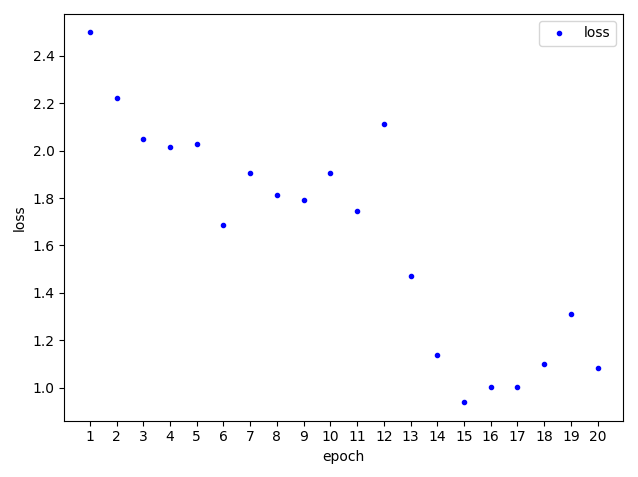
\includegraphics[height=7cm]{./images/loss_decrease.png}
	\caption{Spadek kosztu na głowicy numer 1 na danych treningowych}
	\label{fig:test5}
	\end{figure}

Pozostałym elementom kodu nie udało nam się nic zarzucić. Na dalsze szukanie błędów brakło nam czasu.
